% !TEX spellcheck = en_US



% ~~~~~~~~~~~~~~~~~~~~~~~~~~~~~~~~~~~~~~~ V
% (NC) 2026 Haluk Bingol
% github.com/halukbingol/LaTeX-Templates
%
% Licensees may copy, distribute, display, and perform the work and make derivative works 
% and remixes based on it only for non-commercial purposes. 
% ~~~~~~~~~~~~~~~~~~~~~~~~~~~~~~~~~~~~~~~ A


% v20261029T1800

\documentclass[aspectratio=169,10pt,compress]{beamer}




% ~~~~~~~~~~~~~~~~~~~~~~~~~~~~~~~~~~~~~~~~~~~~~~~~~~~~~~~~~~~~~~~~~ V hblib
	\usepackage{../../hblib/hblibPresentation} % lib presentation: theme, i/N, \hSection, algorithm2e, ...
	\usepackage{../../hblib/hblibCodeoutput} % lib code + output: \lstcode, \lstterminal, ...
	\usepackage{../../hblib/hblibDatastructures} % lib data structures: \hString, \hStack, \hQueue, \hArray
% ~~~~~~~~~~~~~~~~~~~~~~~~~~~~~~~~~~~~~~~~~~~~~~~~~~~~~~~~~~~~~~~~~ A hblib




% +++++++++++++++++++++++++++++++++++++++ V specific
\DontPrintSemicolon % in algorithms
% +++++++++++++++++++++++++++++++++++++++ A specific



\title[Arrays 1D: Junior]{
	One-Dimensional Arrays\\
	Junior
}
\subtitle{
	\cisOOO\ -- Level 3: growing, searching, sorting, performance
}
\author[Erkovan]{Sait Erkovan}

\institute[FCIS]{
	Faculty of Computer and Information Sciences\\
	Yeditepe University
}
\date{{\tiny \hbTimeStamp}}

\begin{document}




% ~~~~~~~~~~~~~~~~~~~~~~~~~~~~~~~~~~~~~~ V frm
\begin{frame}[t,fragile]
	\titlepage
\end{frame}
% ~~~~~~~~~~~~~~~~~~~~~~~~~~~~~~~~~~~~~~ A frm




% ~~~~~~~~~~~~~~~~~~~~~~~~~~~~~~~~~~~~~~ V frm
\begin{frame}[t,fragile] \frametitle{Outline}
	\begin{columns}[T]
		\begin{column}{0.48\textwidth}
			\tableofcontents[sections={1-4}, hideallsubsections]
		\end{column}
		\begin{column}{0.48\textwidth}
			\tableofcontents[sections={5-8}, hideallsubsections]
		\end{column}
	\end{columns}

	\vspace{1em}
	\small Assumes \hCode{array1D-2-sophomore}: \hCode{java.util.Arrays}, copying, tests.
	Here: what arrays cost, and how to make them cheap.
\end{frame}
% ~~~~~~~~~~~~~~~~~~~~~~~~~~~~~~~~~~~~~~ A frm




% ~~~~~~~~~~~~~~~~~~~~~~~~~~~~~~~~~~~~~~ V
\hSection[Grow]{Growing an array}
% ~~~~~~~~~~~~~~~~~~~~~~~~~~~~~~~~~~~~~~ A




% ~~~~~~~~~~~~~~~~~~~~~~~~~~~~~~~~~~~~~~ V frm
\begin{frame}[t,fragile] \frametitle{A growable array: capacity and size}
	\lstcode[basicstyle=\ttfamily\scriptsize, lastline=18]{codeoutput/DynamicArray.java}{Java}

	\small An array cannot grow, so \hCode{makeRoom} makes a new one, twice as long, and copies.
	\hCode{size} counts the elements in use.
\end{frame}
% ~~~~~~~~~~~~~~~~~~~~~~~~~~~~~~~~~~~~~~ A frm




% ~~~~~~~~~~~~~~~~~~~~~~~~~~~~~~~~~~~~~~ V frm
\begin{frame}[t,fragile] \frametitle{Insert and remove: shifting with arraycopy}
	\lstcode[basicstyle=\ttfamily\scriptsize, firstline=20, lastline=30, firstnumber=20]{codeoutput/DynamicArray.java}{Java}

	\begin{center}
		\begin{tikzpicture}
			\hArray[id=a, name={insert(1, 15)}, width=0.65, index=below, unused={4,5}, hot={1,2,3}]{10,20,30,40,0,0}
			\draw[->, colorStop, thick] (a-3.north) to[bend left=50] (a-4.north);
			\draw[->, colorStop, thick] (a-1.north) to[bend left=50] (a-2.north);
			\hArray[id=b, name={remove(0)}, at={(7.6,0)}, width=0.65, index=below, unused={4,5}, hot={1,2,3}]{10,20,30,40,0,0}
			\draw[->, colorStop, thick] (b-1.north) to[bend right=50] (b-0.north);
			\draw[->, colorStop, thick] (b-3.north) to[bend right=50] (b-2.north);
		\end{tikzpicture}
	\end{center}

	\small \hCode{arraycopy} works correctly even when source and destination overlap.
	Insert and remove move up to \hCode{size} elements: $O(n)$.
\end{frame}
% ~~~~~~~~~~~~~~~~~~~~~~~~~~~~~~~~~~~~~~ A frm




% ~~~~~~~~~~~~~~~~~~~~~~~~~~~~~~~~~~~~~~ V frm
\begin{frame}[t,fragile] \frametitle{Watch the capacity}
	\lstcoderightstep[0.5][basicstyle=\ttfamily\scriptsize, firstline=38, firstnumber=38][basicstyle=\ttfamily\scriptsize]{codeoutput/DynamicArray.java}{Java}{codeoutput/DynamicArray.txt}

	\small The capacity jumps 2, 4, 8: most \hCode{add}s are cheap, a few copy everything.
\end{frame}
% ~~~~~~~~~~~~~~~~~~~~~~~~~~~~~~~~~~~~~~ A frm




% ~~~~~~~~~~~~~~~~~~~~~~~~~~~~~~~~~~~~~~ V frm
\begin{frame}[t,fragile] \frametitle{Why double? Count the copies}
	\lstcodedownstep[basicstyle=\ttfamily\scriptsize, firstline=3, lastline=13, firstnumber=3][basicstyle=\ttfamily\scriptsize]{codeoutput/GrowthCost.java}{Java}{codeoutput/GrowthCost.txt}
\end{frame}
% ~~~~~~~~~~~~~~~~~~~~~~~~~~~~~~~~~~~~~~ A frm




% ~~~~~~~~~~~~~~~~~~~~~~~~~~~~~~~~~~~~~~ V frm
\begin{frame}[t,fragile] \frametitle{Amortized cost}
	\begin{columns}[T]
		\begin{column}{0.48\textwidth}
			\textbf{Grow by one}: every add copies all
			\[
				1 + 2 + \dots + (n - 1) = \frac{n (n - 1)}{2}
			\]
			copies: $O(n^{2})$ in total, $O(n)$ per add.
		\end{column}
		\begin{column}{0.48\textwidth}
			\textbf{Double}: copies only at $1, 2, 4, \dots, 2^{k} < n$
			\[
				1 + 2 + 4 + \dots + 2^{k} = 2^{k + 1} - 1 < 2 n
			\]
			copies: $O(n)$ in total, $O(1)$ per add \hDefined{on average}.
		\end{column}
	\end{columns}

	\vspace{1em}
	\begin{block}{Amortized}
		One \hCode{add} may cost $n$ copies, but the expensive ones are rare: spread over all adds,
		the cost per add is a constant. The table: $1\,048\,575 < 2 \cdot 10^{6}$ copies for a million adds.
	\end{block}
\end{frame}
% ~~~~~~~~~~~~~~~~~~~~~~~~~~~~~~~~~~~~~~ A frm




% ~~~~~~~~~~~~~~~~~~~~~~~~~~~~~~~~~~~~~~ V
\hSection[Search]{Searching a sorted array}
% ~~~~~~~~~~~~~~~~~~~~~~~~~~~~~~~~~~~~~~ A




% ~~~~~~~~~~~~~~~~~~~~~~~~~~~~~~~~~~~~~~ V frm
\begin{frame}[t,fragile] \frametitle{Binary search: halve the range}
	Find 23 in a \hEmph{sorted} array. Gray: ruled out. Green: the middle element \hCode{mid}.

	\vspace{0.5em}
	\begin{center}
		\begin{tikzpicture}
			\only<1>{\hArray[id=a, width=0.62, cur={7}]{2,5,8,12,16,23,38,45,56,67,72,81,85,90,94,99}}
			\only<2>{\hArray[id=a, width=0.62, cur={3}, unused={7,...,15}]{2,5,8,12,16,23,38,45,56,67,72,81,85,90,94,99}}
			\only<3>{\hArray[id=a, width=0.62, cur={5}, unused={0,...,3,7,8,9,10,11,12,13,14,15}]{2,5,8,12,16,23,38,45,56,67,72,81,85,90,94,99}}
			\node[font=\small, anchor=west] at (0,-0.6) {%
				\only<1>{lo 0, hi 15, mid 7: $45 > 23$, so hi $\gets$ 6}%
				\only<2>{lo 0, hi 6, mid 3: $12 < 23$, so lo $\gets$ 4}%
				\only<3>{lo 4, hi 6, mid 5: found 23 at index 5, after 3 steps}};
		\end{tikzpicture}
	\end{center}

	\begin{itemize}\small
		\item Every step looks at one element and throws away \hEmph{half} of the rest
		\item $n = 16$: at most 5 steps; a linear search may need 16
		\item Only for sorted arrays: the order tells which half to keep
	\end{itemize}
\end{frame}
% ~~~~~~~~~~~~~~~~~~~~~~~~~~~~~~~~~~~~~~ A frm




% ~~~~~~~~~~~~~~~~~~~~~~~~~~~~~~~~~~~~~~ V frm
\begin{frame}[t,fragile] \frametitle{Binary search in Java}
	\lstcode[basicstyle=\ttfamily\scriptsize, firstline=15, lastline=30, firstnumber=15]{codeoutput/BinarySearch.java}{Java}

	\small Line 19: \hCode{lo + (hi - lo) / 2}, not \hCode{(lo + hi) / 2}. Why: \hCode{array1D-4-senior}.
	\hCode{Arrays.binarySearch} does the same; when the key is absent it returns $-(\mathit{insertion\ point}) - 1$.
\end{frame}
% ~~~~~~~~~~~~~~~~~~~~~~~~~~~~~~~~~~~~~~ A frm




% ~~~~~~~~~~~~~~~~~~~~~~~~~~~~~~~~~~~~~~ V frm
\begin{frame}[t,fragile] \frametitle{How many steps?}
	\begin{columns}[T]
		\begin{column}{0.48\textwidth}
			\lstoutput[basicstyle=\ttfamily\scriptsize]{codeoutput/BinarySearch.txt}
		\end{column}
		\begin{column}{0.48\textwidth}
			The key is not there (1 in $0, 2, 4, \dots$): the worst case for linear search.
			\[
				\text{linear: } n
				\qquad
				\text{binary: at most } \lfloor \log_{2} n \rfloor + 1
			\]
			Ten times more data: linear search is ten times slower,
			binary search needs about 3.3 more steps.
		\end{column}
	\end{columns}

	\vspace{0.5em}
	\begin{alertblock}{Sorting first is not free}
		\small Sorting costs $O(n \log n)$. It pays off when you search the same array many times.
	\end{alertblock}
\end{frame}
% ~~~~~~~~~~~~~~~~~~~~~~~~~~~~~~~~~~~~~~ A frm




% ~~~~~~~~~~~~~~~~~~~~~~~~~~~~~~~~~~~~~~ V
\hSection[Sort]{Sorting}
% ~~~~~~~~~~~~~~~~~~~~~~~~~~~~~~~~~~~~~~ A




% ~~~~~~~~~~~~~~~~~~~~~~~~~~~~~~~~~~~~~~ V frm
\begin{frame}[t,fragile] \frametitle{Selection sort: pick the smallest, swap it forward}
	\begin{columns}[T]
		\begin{column}{0.58\textwidth}
			\lstcode[basicstyle=\ttfamily\scriptsize, firstline=6, lastline=18, firstnumber=6]{codeoutput/SortGrowth.java}{Java}
		\end{column}
		\begin{column}{0.40\textwidth}
			\vspace{0.4em}
			\begin{tikzpicture}
				\only<1>{\hArray[id=a, width=0.6, hot={4}]{64,25,12,22,11}}
				\only<2>{\hArray[id=a, width=0.6, done={0}, hot={2}]{11,25,12,22,64}}
				\only<3>{\hArray[id=a, width=0.6, done={0,1}, hot={3}]{11,12,25,22,64}}
				\only<4>{\hArray[id=a, width=0.6, done={0,1,2}, hot={3}]{11,12,22,25,64}}
				\only<5>{\hArray[id=a, width=0.6, done={0,...,4}]{11,12,22,25,64}}
				\node[font=\scriptsize, anchor=west, text width=4.5cm] at (0,-0.7) {%
					\only<1>{$i = 0$: smallest is 11 (index 4); swap with 64}%
					\only<2>{$i = 1$: smallest of the rest is 12; swap}%
					\only<3>{$i = 2$: smallest of the rest is 22; swap}%
					\only<4>{$i = 3$: 25 is already in place}%
					\only<5>{sorted: the last one is in place by itself}};
			\end{tikzpicture}

			\vspace{1.2em}
			\small Pink: sorted part. Yellow: the smallest of the rest.
			Comparisons: $(n - 1) + (n - 2) + \dots + 1 = n (n - 1) / 2$.
		\end{column}
	\end{columns}
\end{frame}
% ~~~~~~~~~~~~~~~~~~~~~~~~~~~~~~~~~~~~~~ A frm




% ~~~~~~~~~~~~~~~~~~~~~~~~~~~~~~~~~~~~~~ V frm
\begin{frame}[t,fragile] \frametitle{$O(n^{2})$ against $O(n \log n)$, measured}
	\begin{columns}[T]
		\begin{column}{0.52\textwidth}
			\lstoutput[basicstyle=\ttfamily\scriptsize]{codeoutput/SortGrowth.txt}

			\footnotesize One run, best of 3 per size, after a warm-up;
			your numbers will differ, the ratios will not.
		\end{column}
		\begin{column}{0.44\textwidth}
			\begin{itemize}\small
				\item Double $n$: selection sort takes about \hEmph{4 times} longer
				\item \hCode{Arrays.sort} only about twice
				\item At $n = 80\,000$: hundreds of times faster
			\end{itemize}
		\end{column}
	\end{columns}

	\vspace{0.5em}
	\begin{block}{What Arrays.sort uses (JDK 21 documentation)}
		\small Primitive arrays: \emph{Dual-Pivot Quicksort} (Yaroslavskiy, Bentley, Bloch), $O(n \log n)$.
		Object arrays: a \emph{stable} merge sort adapted from TimSort; equal elements keep their order.
	\end{block}
\end{frame}
% ~~~~~~~~~~~~~~~~~~~~~~~~~~~~~~~~~~~~~~ A frm




% ~~~~~~~~~~~~~~~~~~~~~~~~~~~~~~~~~~~~~~ V
\hSection[Techniques]{Array techniques}
% ~~~~~~~~~~~~~~~~~~~~~~~~~~~~~~~~~~~~~~ A




% ~~~~~~~~~~~~~~~~~~~~~~~~~~~~~~~~~~~~~~ V frm
\begin{frame}[t,fragile] \frametitle{A counting array: the value is the index}
	\lstcoderightstep[0.66][basicstyle=\ttfamily\scriptsize]{codeoutput/Histogram.java}{Java}{codeoutput/Histogram.txt}

	\small One pass, no search: \hCode{counts[s / 10]++} finds the right counter directly.
\end{frame}
% ~~~~~~~~~~~~~~~~~~~~~~~~~~~~~~~~~~~~~~ A frm




% ~~~~~~~~~~~~~~~~~~~~~~~~~~~~~~~~~~~~~~ V frm
\begin{frame}[t,fragile] \frametitle{Prefix sums: range totals in O(1)}
	\lstcoderightstep[0.66][basicstyle=\ttfamily\scriptsize]{codeoutput/PrefixSums.java}{Java}{codeoutput/PrefixSums.txt}

	\[
		p_{0} = 0, \quad p_{i + 1} = p_{i} + a_{i}
		\qquad\Rightarrow\qquad
		a_{lo} + \dots + a_{hi} = p_{hi + 1} - p_{lo}
	\]
\end{frame}
% ~~~~~~~~~~~~~~~~~~~~~~~~~~~~~~~~~~~~~~ A frm




% ~~~~~~~~~~~~~~~~~~~~~~~~~~~~~~~~~~~~~~ V frm
\begin{frame}[t,fragile] \frametitle{Two pointers: walk from both ends}
	\begin{columns}[T]
		\begin{column}{0.49\textwidth}
			\lstcode[basicstyle=\ttfamily\scriptsize, firstline=5, lastline=15, firstnumber=5]{codeoutput/TwoPointers.java}{Java}
		\end{column}
		\begin{column}{0.49\textwidth}
			\lstcode[basicstyle=\ttfamily\scriptsize, firstline=17, lastline=28, firstnumber=17]{codeoutput/TwoPointers.java}{Java}
		\end{column}
	\end{columns}

	\uncover<2->{\lstoutput[basicstyle=\ttfamily\scriptsize]{codeoutput/TwoPointers.txt}}

	\small In place, $n / 2$ steps, no second array. The output: \hCode{\{1, 2, 3, 4, 5\}} reversed,
	then two palindrome tests.
\end{frame}
% ~~~~~~~~~~~~~~~~~~~~~~~~~~~~~~~~~~~~~~ A frm




% ~~~~~~~~~~~~~~~~~~~~~~~~~~~~~~~~~~~~~~ V frm
\begin{frame}[t,fragile] \frametitle{Varargs: \texttt{int...} is an \texttt{int[]}}
	\lstcoderightstep[0.66][basicstyle=\ttfamily\scriptsize]{codeoutput/Varargs.java}{Java}{codeoutput/Varargs.txt}
\end{frame}
% ~~~~~~~~~~~~~~~~~~~~~~~~~~~~~~~~~~~~~~ A frm




% ~~~~~~~~~~~~~~~~~~~~~~~~~~~~~~~~~~~~~~ V
\hSection[Speed]{Memory and performance}
% ~~~~~~~~~~~~~~~~~~~~~~~~~~~~~~~~~~~~~~ A




% ~~~~~~~~~~~~~~~~~~~~~~~~~~~~~~~~~~~~~~ V frm
\begin{frame}[t,fragile] \frametitle{Neighbors are cheap: memory locality}
	\lstcodedownstep[basicstyle=\ttfamily\scriptsize, lastline=11][basicstyle=\ttfamily\scriptsize]{codeoutput/Locality.java}{Java}{codeoutput/Locality.txt}

	\small \uncover<2->{Same additions, same sum. The processor loads memory in \emph{cache lines}
	(typically 64 bytes, 16 \hCode{int}s): stride 1 uses all 16, stride 16 uses one per load.}
\end{frame}
% ~~~~~~~~~~~~~~~~~~~~~~~~~~~~~~~~~~~~~~ A frm




% ~~~~~~~~~~~~~~~~~~~~~~~~~~~~~~~~~~~~~~ V frm
\begin{frame}[t,fragile] \frametitle{Measuring memory}
	\lstcode[basicstyle=\ttfamily\scriptsize, firstline=8, lastline=26, firstnumber=8]{codeoutput/Boxing.java}{Java}
\end{frame}
% ~~~~~~~~~~~~~~~~~~~~~~~~~~~~~~~~~~~~~~ A frm




% ~~~~~~~~~~~~~~~~~~~~~~~~~~~~~~~~~~~~~~ V frm
\begin{frame}[t,fragile] \frametitle{int[] or Integer[]?}
	\begin{columns}[T]
		\begin{column}{0.52\textwidth}
			\begin{tikzpicture}
				\hArray[id=p, name={int[]}, width=0.6]{7,3,9,1}
				\hArray[id=q, name={Integer[]}, at={(0,-1.3)}, width=0.6, font=\tiny]{,,,}
				\foreach \k/\v in {0/7,1/3,2/9,3/1} {
					\node[draw, rounded corners=2pt, font=\ttfamily\scriptsize, fill=colorHead!40] (o\k) at (\k*0.9+0.3,-2.5) {\v};
					\fill (q-\k.center) circle (1.2pt);
					\draw[href] (q-\k.center) -- (o\k.north);
				}
			\end{tikzpicture}
		\end{column}
		\begin{column}{0.44\textwidth}
			\uncover<2->{\lstoutput[basicstyle=\ttfamily\scriptsize]{codeoutput/Boxing.txt}}
		\end{column}
	\end{columns}

	\begin{itemize}\small
		\item \hCode{int[]}: 4 bytes per element, side by side
		\item \hCode{Integer[]}: an arrow per element \emph{plus} an object per value, scattered in memory
		\item<2-> 10 million values: about 5 times the memory (a rough measurement; it depends on the JVM)
	\end{itemize}
\end{frame}
% ~~~~~~~~~~~~~~~~~~~~~~~~~~~~~~~~~~~~~~ A frm




% ~~~~~~~~~~~~~~~~~~~~~~~~~~~~~~~~~~~~~~ V frm
\begin{frame}[t,fragile] \frametitle{Measuring speed honestly}
	\begin{itemize}
		\item The JIT compiler optimizes code \emph{while} it runs: the first runs are slower.
		      \hCode{SortGrowth} warms up first and keeps the best of 3
		\item Other programs, power saving and garbage collection add noise: repeat, compare ratios
		\item The JIT may remove work whose result is never used: print or return the result
		      (\hCode{Locality} prints the sum)
		\item For serious measurements use a benchmark harness such as JMH
	\end{itemize}


% +++++++++++++++++++++++++++++++++++++++ V lst
%: -Lst. jmh
\begin{lstlisting}[style=codesnippet, language=Java]
@Benchmark
public long sumSequential() { return Locality.sumWithStride(data, 1); }
\end{lstlisting}
% +++++++++++++++++++++++++++++++++++++++ A lst


	\hRemark{Not run here}: JMH needs a Maven or Gradle project.
\end{frame}
% ~~~~~~~~~~~~~~~~~~~~~~~~~~~~~~~~~~~~~~ A frm




% ~~~~~~~~~~~~~~~~~~~~~~~~~~~~~~~~~~~~~~ V
\hSection[Records]{Arrays in larger programs}
% ~~~~~~~~~~~~~~~~~~~~~~~~~~~~~~~~~~~~~~ A




% ~~~~~~~~~~~~~~~~~~~~~~~~~~~~~~~~~~~~~~ V frm
\begin{frame}[t,fragile] \frametitle{Parallel arrays or one array of records?}
	\lstcoderightstep[0.66][basicstyle=\ttfamily\scriptsize, firstline=4, firstnumber=4]{codeoutput/Records.java}{Java}{codeoutput/Records.txt}

	\footnotesize \uncover<2->{Sorting \hCode{scores} alone broke the pairs (Ayşe shows Zeynep's 64); a \hCode{record} keeps them together.}
\end{frame}
% ~~~~~~~~~~~~~~~~~~~~~~~~~~~~~~~~~~~~~~ A frm




% ~~~~~~~~~~~~~~~~~~~~~~~~~~~~~~~~~~~~~~ V
\hSection[Summary]{Summary}
% ~~~~~~~~~~~~~~~~~~~~~~~~~~~~~~~~~~~~~~ A




% ~~~~~~~~~~~~~~~~~~~~~~~~~~~~~~~~~~~~~~ V frm
\begin{frame}[t,fragile] \frametitle{Cheat sheet: what each operation costs}


% +++++++++++++++++++++++++++++++++++++++ V tbl
%: -Tbl. costs
\begin{table}
		\small
		\begin{tabular}{@{}L{0.38\textwidth}L{0.22\textwidth}L{0.30\textwidth}@{}}
			\toprule
			\textbf{Operation} & \textbf{Cost} & \textbf{Remark} \\
			\midrule
			\hCode{a[i]}, \hCode{a[i] = x}      & $O(1)$          & address arithmetic \\
			add at the end (doubling)           & $O(1)$ amortized & now and then $O(n)$ \\
			insert, remove at index             & $O(n)$          & shifting \\
			linear search                       & $O(n)$          & any array \\
			binary search                       & $O(\log n)$     & sorted array only \\
			selection sort                      & $O(n^{2})$      & simple, slow \\
			\hCode{Arrays.sort}                 & $O(n \log n)$   & use this one \\
			range sum with prefix sums          & $O(1)$          & after $O(n)$ preparation \\
			\bottomrule
		\end{tabular}
\end{table}%
% +++++++++++++++++++++++++++++++++++++++ A tbl


\end{frame}
% ~~~~~~~~~~~~~~~~~~~~~~~~~~~~~~~~~~~~~~ A frm




% ~~~~~~~~~~~~~~~~~~~~~~~~~~~~~~~~~~~~~~ V frm
\begin{frame}[t,fragile] \frametitle{Exercises and projects}
	\textbf{Exercises}
	\begin{enumerate}\small
		\item Give \hCode{DynamicArray} a \hCode{get(i)} that throws an exception for $i \ge$ \hCode{size}
		      (not only for $i \ge$ capacity). Why does it matter?
		\item Count the comparisons of selection sort for $n = 10, 100, 1000$ and compare with $n (n - 1) / 2$.
		\item Write insertion sort. Measure it on random and on already sorted arrays. Explain the difference.
		\item With prefix sums, find the 7-day period with the most steps in a year of data in $O(n)$.
	\end{enumerate}

	\textbf{Projects}
	\begin{itemize}\small
		\item An \hCode{IntList} class with \hCode{add}, \hCode{insert}, \hCode{remove}, \hCode{get}, \hCode{indexOf},
		      JUnit tests, and a growth factor you can change; measure 1.5 against 2
		\item A ``top $k$'' of exam scores without sorting everything: keep a small sorted array
	\end{itemize}
\end{frame}
% ~~~~~~~~~~~~~~~~~~~~~~~~~~~~~~~~~~~~~~ A frm




% ~~~~~~~~~~~~~~~~~~~~~~~~~~~~~~~~~~~~~~ V frm
\begin{frame}[t,fragile] \frametitle{References}
	\small Searching and sorting: CLRS \cite{cormen2022introduction}; Knuth \cite{knuth1973artv1};
	\hCode{java.util.Arrays}, JDK 21 API documentation.

	\vspace{1em}
	\setbeamertemplate{bibliography item}[text]
	\bibliographystyle{IEEEtran}
	\tiny\bibliography{../../hblib/hblibDataStructures}
\end{frame}
% ~~~~~~~~~~~~~~~~~~~~~~~~~~~~~~~~~~~~~~ A frm




% ~~~~~~~~~~~~~~~~~~~~~~~~~~~~~~~~~~~~~~ V frm
\begin{frame}[t,fragile]
	\begin{center}
		\vspace{4cm}
		\hRemark{\Huge Questions?}
	\end{center}
\end{frame}
% ~~~~~~~~~~~~~~~~~~~~~~~~~~~~~~~~~~~~~~ A frm



\end{document}
